% Physics Homework Template
% Useful for completing homework questions from the textbook.
\documentclass[11pt]{homework}
\usepackage{siunitx}
\usepackage{amsmath}
\usepackage{tikz}
\usepackage{pgfplots}
\pgfplotsset{compat=1.18}

\newcommand{\hwname}{Corbin Hibler}
\newcommand{\hwemail}{c-hibler@onu.edu}
\newcommand{\hwtype}{Ch. 3 HW}
\newcommand{\hwnum}{}
\newcommand{\hwclass}{PHYS 2311}
\newcommand{\hwlecture}{0}
\newcommand{\hwsection}{Z}

\begin{document}
\maketitle

% Problems
\renewcommand{\questiontype}{Problem}
\setcounter{questionCounter}{0}

\question
\[
\Delta \vec{r}=\vec{r}_{f}-\vec{r}_{i}
\]\[
\vec{v}_1 = -245\hat{i} + 0\hat{j}
\]\[
\vec{v}_2=118 \cos 225\hat{i}+118 \cos 225\hat{j}
\] \[
\vec{v}_2=-83.4\hat{i}-83.4\hat{j}
\] \[
\vec{v}_{1}+\vec{v}_{2}=(v_{1x}+v_{2x})\hat{i}+(v_{1y}+v_{2y})\hat{j}
\] \[
\vec{v}_{1}+\vec{v}_{2}=(-245-83.4)\hat{i}+(0-83.4)\hat{j} = -328\hat{i}-83.4\hat{j}
\] \[
|\vec R| = \sqrt{(-328)^2+(-83.4)^2} = \boxed{\qty{339}{km}}
\] \[
\theta=\arctan\left( \frac{A_{y}}{A_{x}} \right)
\] 
\[
    \theta= \arctan\left(\frac{-328}{-83.4}\right) =\boxed{14.3^{\circ}\mbox{ south of west}}
\] 
\centering
\begin{tikzpicture}
    % Draw the number line (horizontal axis)
    \draw[->](-5,0)  node[left] {West}  -- (1,0) node[right] {East}; % X-axis with label
    \draw[->] (0,-3) node[below] {South}-- (0,1) node[above] {North}; % Y-axis with label
    
    % Draw the westward arrow
    \draw[->, thick] (0,0) -- (-2.45,0) node[midway, above] {245 km};

    % Draw the southwest arrow (45 degrees from west)
    \draw[->, thick] (-2.45,0) -- (-3.04,-0.59) node[midway, left] {118 km};
    \draw[->, thick] (0,0) -- (-3.04,-0.59) node[midway, below right] { km};

\end{tikzpicture}

           
\setcounter{questionCounter}{2}
\question
\[
|\vec{R}| = \sqrt{(9.40)^2+(-6.80)^2}= \boxed{\qty{11.6}{units}} 
\]\[
\theta = \arctan \left( \frac{-6.80}{9.40} \right) = \boxed{\qty{-35.9}{\degree}}
\] 
 
\setcounter{questionCounter}{5}
\question
\begin{alphaparts}
\questionpart
\[
\vec{v}_{1}=6.2\hat{i}+0\hat{j}
\] \[
\vec{v}_{2}=8.1\cos 55 \hat{i} + 8.1\sin 55 \hat{j}
\] \[
\vec{v}_{2}=4.646\hat{i}+6.635\hat{j}
\]

\questionpart
\[
\vec{v}_{1}+\vec{v}_{2}=(v_{1x}+v_{2x})\hat{i}+(v_{1y}+v_{2y})\hat{j}
\]
\[
(6.2+4.646)\hat{i}+(0+6.635)\hat{j} = 10.85\hat{i}+6.64\hat{j}
\]
\[\vec{R}=10.85\hat{i}+6.64\hat{j}\]
\[
    R=|\vec{R}|=\sqrt{ 10.85^2+6.64^2 }=\boxed{\qty{12.72}{units}}
    \]\[
    \theta=\arctan\left( \frac{6.64}{10.85} \right)=\boxed{\qty{31.48}{\degree}}
\]
\end{alphaparts} 
\question
\begin{alphaparts}
    \questionpart
    \[
        \vec{C}=\vec{A}+\vec{B}
    \] \[
        \vec{C}=6.8\hat{i}-5.5\hat{i}
    \] \[
    \vec{C}=1.3\hat{i} \mbox{ units in +x direction}
    \] 
    \questionpart \[
        \vec{C}=\vec{A}-\vec{B}
    \] \[
    \vec{C}=6.8\hat{i}-(-5.5\hat{i})
    \] \[
    \vec{C}=12.3\hat{i}\mbox{ units in +x direction}
    \] 
    \questionpart \[
        \vec{C}=\vec{B}-\vec{A}
    \] \[
    \vec{C}=-5.5\hat{i}-6.8\hat{i}
    \] \[
\vec{C}=-12.3\hat{i}\mbox{ units in -x direction}\]
\end{alphaparts}

\setcounter{questionCounter}{9}
\question
\begin{alphaparts}
    \questionpart
    \[
        \vec{A}=42.0 \cos 28\hat{i}+42.0 \sin28.0\hat{j}
    .\] \[
    \vec{A}=37.1\hat{i}+19.7\hat{j}
    .\] \[
    \vec{B}=-29.7\cos56.0\hat{i}+29.7\sin56.0\hat{j}
    .\] \[
    \vec{B}=-16.6\hat{i}+24.6\hat{j}
    .\] \[
    \vec{C}=31.0\cos90-31.0\sin90
    .\] \[
    \vec{C}=0\hat{i}-31.0\hat{j}
    .\] \[
    \vec{A}+\vec{B}+\vec{C}
    .\] \[
    (\vec{A}_x+\vec{B}_x+\vec{C}_x)\hat{i}+(\vec{A}_y+\vec{B}_y+\vec{C}_y)\hat{j}
    .\] \[
    (37.1-16.6+0)\hat{i}+(19.7+24.6-31.0)\hat{j}
    .\] \[
    \boxed{20.5\hat{i}+13.3\hat{j}}
    .\] 
    \questionpart
    \[
        |\vec{R}|=\sqrt{(20.5)^2+(13.3)^2}=\boxed{\qty{24.4}{units}} 
    .\] \[
    \theta = \arctan(\frac{13.3}{20.5})=\boxed{\qty{33.0}{\degree}}
    .\] 
\end{alphaparts}
\question
\begin{alphaparts}
    \questionpart
    \[
        \vec{B}-\vec{A}
    .\] \[
    (-16.6-37.1)\hat{i}+(24.6-19.7)\hat{j}
    .\] \[
    -53.7\hat{i}+4.9\hat{j}
    .\] \[
    |\vec{R}|=\sqrt{(-53.7)^2+(4.9)^2}=\boxed{\qty{53.9}{units}}
    .\] \[
    \theta=\arctan \left(\frac{4.9}{-53.9}\right)=180-5.2=\boxed{\qty{174.8}{\degree}}
    .\] 
    \questionpart
    \[
        \vec{A}-\vec{B}
    .\] \[
    (37.1-(-16.6))\hat{i}+(19.7-24.6)\hat{j}
    .\] \[
    53.7\hat{i}-4.9\hat{j}
    .\] \[
    |\vec{R}|=\sqrt{(53.7)^2+(-4.9)^2}=\boxed{\qty{53.9}{units}}
    .\] \[
    \theta=\arctan \left(\frac{-4.9}{53.9}\right)=360-5.2=\boxed{\qty{354.8}{\degree}}
    .\] 
    \questionpart
They are the opposites of each other, exactly \qty{180}{\degree} apart.
\end{alphaparts}
\setcounter{questionCounter}{18}
\question
\[
    \vec{r}=(9.60t\hat{i}+6.45\hat{j}-1.50t^2\hat{k})
.\] \[
\vec{v}=\left(\frac{\mathrm{d}}{\mathrm{dt}}(9.60t)\hat{i}+\frac{\mathrm{d}}{\mathrm{dt}}(6.45)\hat{j}-\frac{\mathrm{d}}{\mathrm{dt}}(1.50t^2)\hat{k} \right)
.\] \[
\vec{v}=\boxed{(9.60\hat{i}+0\hat{j}-3t\hat{k})\unit{m/s}}
.\] \[
\vec{a}=\left(\frac{\mathrm{d}}{\mathrm{dt}}(9.60)\hat{i}+0\hat{j}-\frac{\mathrm{d}}{\mathrm{dt}}(3t)\hat{k}\right)
.\] \[
\vec{a}=\boxed{(0\hat{i}+0\hat{j}-3\hat{k})\unit{m/s^2}}
.\] 
\question
\[
\Delta \vec{r}=\vec{r}_{f}-\vec{r}_{i}
.\] \[
=(9.60(3.00)\hat{i}+6.45\hat{j}-1.50(3.00)^2\hat{k})-(9.60\hat{i}+6.45\hat{j}-1.50\hat{k})
.\] \[
=(28.8\hat{i}+6.45\hat{j}-13.5\hat{k})-(9.60\hat{i}+6.45\hat{j}-1.50\hat{k})
.\] \[
=(19.2\hat{i}-12.0\hat{k})
.\] \[
|\vec{R}|=\sqrt{(19.2)^2+(-12.0)^2}=\qty{22.6}{m} 
.\] \[
\vec{v}_{avg} =\frac{\Delta \vec{r}}{\Delta t} = \frac{22.6}{3.00-1.00}=\boxed{\qty{11.3}{m/s}}
.\] \[
\vec{v}_{inst}=(9.60\hat{i}-3t\hat{k})
.\] \[
=(9.60\hat{i}-3(2.00)\hat{k})
.\] \[
=9.60\hat{i}-6\hat{k}
.\] \[
\sqrt{(9.60)^2+(-6)^2}=\boxed{\qty{11.3}{m/s}} 
.\] 

\setcounter{questionCounter}{22}
\question
\begin{alphaparts}
    \questionpart
    \[
    \vec{a}=1.80\cos330\hat{i}+1.80\sin330\hat{j}
    .\] \[
    =1.56\hat{i}-0.90\hat{j}
    .\] \[
    \boxed{\qty{-0.90}{m/s^2\hat{j}}}
    .\] 
    \questionpart
    \[
    \vec{r}_{f}=\vec{r}_{i}+\vec{v}_{i}t+\frac{1}{2}\vec{a}t^2
    .\] \[
    0=125+\frac{1}{2}(-0.90)t^2
    .\] \[
    -125=-0.45t^2
    .\] \[
    \sqrt{\frac{-125}{-0.45}}=t=\boxed{\qty{16.7}{s}} 
    .\] 
\end{alphaparts}
\question
\[
    S_{avg} = \frac{11.5}{5.5}=\boxed{\qty{2.09}{km/h}}
\]\[
\vec{A}=8.0\hat{i}+0.85\hat{j}
.\]  \[
A=\sqrt{(8.0)^2+(0.85)^2}=8.05km=\Delta r 
.\] \[
v_{avg}=\frac{\Delta r}{\Delta t}=\frac{8.05}{5.5}=\boxed{\qty{1.46}{km/h}}
.\] \[
\theta =\arctan\left(\frac{0.85}{8.0}\right)=\boxed{\qty{6.06}{\degree}}
.\] 
\setcounter{questionCounter}{31}
\question
\[
x(t)=x_i+v_it
.\] \[
x(t)=3.0t
.\] \[
y(t)=y_i+v_it-\frac{g}{2}t^2
.\] \[
y(t)=7.5 - \frac{g}{2}t^2=0
.\] \[
\sqrt{\frac{7.5}{\frac{g}{2}}}=t=\qty{1.24}{s} 
.\] \[
x(1.24)=3.0(1.24)=\boxed{\qty{3.71}{m}}
.\] 
\question
\[
    y_f=y_i+v_it-\frac{g}{2}t^2
.\] \[
0=y_i-\frac{g}{2}(3.5)^2
.\] \[
y_i=\frac{g}{2}(3.5)^2=\boxed{\qty{60}{m}}
.\] \[
x_f=x_i+v_it
.\] \[
x_f=(2.5)(3.5)=\boxed{\qty{8.8}{m}}
.\] 

\setcounter{questionCounter}{36}
\question
\[
    R=\frac{v_i^2\sin(2\theta)}{g}
.\] \[
2.5=\frac{(6.5)^2\sin(2\theta)}{9.80}
.\] \[
\theta=\frac{35.4}{2}=\boxed{\qty{17.7}{\degree}}
.\] \[
90-17.7=\boxed{\qty{72.3}{\degree}}
.\] 
There is a flat angle and a steep angle from which the water hose can spray at and reach the same place. Algebraically, the $\arcsin$ function will usually give two answers.

\centering
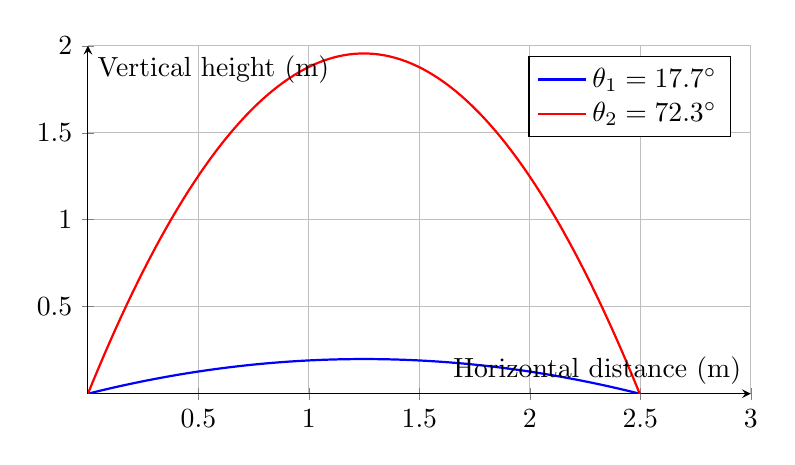
\begin{tikzpicture}
\begin{axis}[
    xlabel={Horizontal distance (m)},
    ylabel={Vertical height (m)},
    axis lines=middle,
    grid=both,
    xmin=0, xmax=3, % Adjust as necessary for better fit
    ymin=0, ymax=2, % Adjust as necessary
    samples=100,
    legend pos=north east,
    width=10cm, height=6cm
]

% Parameters
\pgfmathsetmacro{\v}{6.5} % initial velocity in m/s
\pgfmathsetmacro{\g}{9.8} % gravity in m/s^2

% First trajectory (theta1 = 17.7 degrees)
\pgfmathsetmacro{\thetaone}{17.7}
\addplot[
    domain=0:2.5, 
    thick, 
    blue, 
]
{ x*tan(\thetaone) - (\g/(2*\v^2*cos(\thetaone)^2)) * x^2 };
\addlegendentry{$\theta_1 = 17.7^\circ$};

% Second trajectory (theta2 = 72.3 degrees)
\pgfmathsetmacro{\thetatwo}{72.3}
\addplot[
    domain=0:2.5, 
    thick, 
    red, 
]
{ x*tan(\thetatwo) - (\g/(2*\v^2*cos(\thetatwo)^2)) * x^2 };
\addlegendentry{$\theta_2 = 72.3^\circ$};

\end{axis}
\end{tikzpicture}

\question
\[
    t_{up}=1.7s, t_{down}=1.7s
.\] \[
v_f=v_i-gt_{up}
.\] \[
0=v_i-(9.80)(1.7)
.\] \[
v_i=\qty{16.7}{m/s}
.\] \[
R_{max}=\frac{v_i^2\sin(2(45))}{g}
.\]  \[
R_{max}=\frac{(16.7)^2\sin(2(45))}{9.80} = \boxed{\qty{28.5}{m}}
.\] 
\question
\begin{alphaparts}
    \questionpart
    \[
        \vec{v}_{iy}=v_i\sin\theta=38.8\sin(42.2)=\qty{26.06}{m/s}
    .\] \[
    v_f^2=v_i^2+2g(y_f-y_i)
    .\] \[
    y_f=\frac{v_i^2}{2g}=\frac{(26.06)^2}{2(9.80)}=\boxed{\qty{34.7}{m}}
    .\] 
    \questionpart
    \[
        v_f=v_i+gt_{up}
    .\] \[
    t_{up}=\frac{v_f-v_i}{g}
    .\] \[
    t=2t_{up}=\frac{2(v_f-v_i)}{g}=\frac{2(v_i)}{g}=\frac{2(26.06)}{9.80}=\boxed{\qty{5.32}{s}}
    .\] 
    \questionpart
    \[
        v_{ix}=v_i\cos\theta=38.8\cos42.2=\qty{28.74}{m/s}
    .\] \[
    R=v_{ix}t
    .\] \[
    R=(28.74)(5.32)=\boxed{\qty{152.9}{m}}
    \]
    \questionpart
    \[
        t=\qty{1.50}{s}
    .\] \[
    v_y=v_{iy}-gt
    .\] \[
    v_y=(26.06)-(9.80)(1.50)=\qty{11.36}{m/s}
    .\] \[
    v_x=v_{0x}
    .\] \[
    v=\sqrt{v_x^2+v_y^2} 
    .\] \[
    v=\sqrt{(28.74)^2+(11.36)^2}=\boxed{\qty{30.91}{m/s}} 
    .\] 

\end{alphaparts}
\end{document}
